\RequirePackage[OT1]{fontenc}
\documentclass[conference]{../../setup/IEEEtran}

\usepackage[papersize={8.5in,11in}, left=0.75in, right=0.75in, top=0.8in, bottom=0.8in]{geometry}


\ifCLASSINFOpdf

\else

\fi

\hyphenation{op-tical net-works semi-conduc-tor}

\usepackage[utf8]{inputenc}

\usepackage{lettrine}
\usepackage{amsmath}
\usepackage{multirow}
\usepackage{graphicx}
\usepackage{epstopdf}
%\usepackage{caption}
%


\usepackage{listings}

\usepackage{placeins}
\usepackage{float}
\usepackage{tabularx,colortbl}
\usepackage{algorithm2e}

%Include some predefined commands 

\usepackage{xcolor}
\definecolor{fondtitre}{rgb}{0.20,0.43,0.09}  % vert fonce
\definecolor{coultitre}{rgb}{0.41,0.05,0.05}  % marron
\def\blue#1{\textcolor{beamer@blendedblue}{#1}}
\definecolor{beamer@blendedblue}{HTML}{404bbf}
\def\red#1{\textcolor{red}{#1}}

%\captionsetup[table]{skip=10pt}

\usepackage{color, colortbl}
	\definecolor{mygray}{rgb}{0.5,0.5,0.5}
	\definecolor{mygreen}{rgb}{0,0.6,0}
	\definecolor{gray75}{gray}{0.75}
	\definecolor{marshalcolor}{rgb}{0.93,0.33,0.93} % MARSHAL blue
	\definecolor{draftcolor}{rgb}{0.86,0.86,0.86} % MARSHAL draft color
	\definecolor{darkraspberry}{rgb}{0.53, 0.15, 0.34}

\newcommand{\Equation}[2]{
	\begin{equation}\label{eq:#1}
		#2
	\end{equation}
}

\newcommand{\Table}[4]{
	\begin{table}[h!]
	\begin{center}
		\begin{tabular}{#1}\hline
			#4
		\end{tabular}
		\caption{\label{table:#2} #3.}
	\end{center}
	\end{table}
}


\begin{document} 


%
% To add Footer
% You can use it

\newcommand{\MYfooter}{\smash{
\hfil\parbox[t][\height][t]{\textwidth}{\centering
\thepage}\hfil\hbox{}}}

\makeatletter


\makeatother
% make changes take effect
\pagestyle{headings}
% adjust as needed
\addtolength{\footskip}{0\baselineskip}
\addtolength{\textheight}{-1\baselineskip}


%
% paper title
% can use linebreaks \\ within to get better formatting as desired
\title{IoT-based Urban Traffic-Light Control:  Modelling, Prototyping and MQTT Evaluation}


% Possible titles are: 

%Evaluating QoS in IoT for Modelled and Prototyped Urban Traffic-Light Control

% Evaluation of MQTT for Modelled and Prototyped of IoT-based Urban Traffic-Light Control 

%Performance Assessment of MQTT for Modelled and Prototyped Urban Traffic-Light Control

%Evaluating QoS in IoT for a Modeled and a Prototyped Urban Traffic-Light Control}

%LG: Je propose le titre: A scalable wireless Urban Traffic Light Control IoT system
\author{

\IEEEauthorblockN{
Rafik Zitouni$^{\ddagger}$, Jérémy Petit$^{\ddagger}$, Aghiles Djoudi $^{\ddagger}$ $^{\star}$ and Laurent George$^{\star}$
}

\IEEEauthorblockA{
  ECE Paris$^{\ddagger}$, SIC Laboratory, 37 Quai de Grenelle, 75015 Paris, France\\
  LIGM/ESIEE Paris$^{\star}$, 5 boulevard Descartes, Cité Descartes, Champs-sur-Marne, France\\
Email:   rafik.zitouni@ece.fr, jeremy.petit@ece.fr, aghilesdjoudi@gmail.com, laurent.george@esiee.fr }


}

\maketitle

% ---------------------------------------------------------------------------------------------------------------------
% ------------------------------------------------------------ ABSTRACT -----------------------------------------------
% ---------------------------------------------------------------------------------------------------------------------


\begin{abstract}
%\boldmath

% Problem
Most traffic light's control systems in smart cities are wired and have a semi-static behavior.
They are time-based, with pre-configured pattern and expensive cameras.
% Existing solutions
Although traffic lights can communicate wirelessly with incoming vehicles, they are less adapted to an urban environment. If we consider light signs as an Internet of Things (IoT) network, one issue is to model thoroughly the change of signs' states and the Quality of Service (QoS) of this network.
%System with new applications needs the interoperability between all wireless networks with delay aware of data exchange.
% Our method and results
In this paper, we propose an Urban Traffic Light Control based on an IoT network architecture (IoT-UTLC).
The objective is to interconnect both roads' infrastructures and traffic lights through an IoT Cloud platform.
We designed our IoT-UTLC by selecting motes and protocols of wireless sensor network (WSN).
Message Queuing Telemetry Transport (MQTT) protocol has been integrated to manage QoS.
It enables lights to adapt remotely to any situation and smoothly interrupt traffic light's classic cycles.
%Our experimental results show that the MQTT protocol is efficient when the packets rate exceeds 35\% of traffic flow, it reduces traffic delay up to 0.05s at 90\% of congestion.
After verification and validation of our solution using a UPPAAL model checker,
	our system has been prototyped. Motes' functions have been implemented on Contiki OS and connected through a 6LoWPAN/IEEE 802.15 network.
Time-stamping messages have been performed throughout the system to evaluate the MQTT protocol with different QoS levels.
In our experiments, we measured the Round-trip delay time (RTT) of messages exchanged between the WSN and IoT Cloud. The results show that MQTT decreases the RTT when the Cumulative Distributed Function (CDF) of generated messages exceeds 35\%.
 
\end{abstract}

\begin{IEEEkeywords} Internet of Things (IoT),  Wireless Sensor Networks (WSN), Smart Cities, Traffic Lights Control, IoT Cloud Platform, 6LoWPAN, Contiki OS, QoS, MQTT, UPPAAL
\end{IEEEkeywords}


\IEEEpeerreviewmaketitle



\section{Introduction}

% 1) Motivation

According to the French agency of statistics on roads' accidents, 12\%  of them happen in intersections caused by the non-compliance to traffic rules. 23\% of them led to hospitalization in which 14\% are fatal \cite{Routiere2015}. Urban traffic light are one possible solution to regulate vehicle flows at intersections. However, a static cycle of traffic lights (or lights signs) has a direct impact on traffic jams, particularly when an emergency vehicle must cross through as quickly as possible. A long period at red or green light might impact the fluidity of the city traffic. 
% 4) Proposition + what is in our work that differ with existing solutions
The Internet of Things (IoT) and Everything (IoE) can be a solution to adapt traffic light control to traffic density. It allows different connected objects to interact and exchange data on rouds, vehicles and pedestrians, etc. Furthermore, the IoT is one possible solution for interoperability between heterogeneous wired/wireless networks. 
%
%The exponential growth of 5G networks and the development of IoT that will greatly come with it,
%	would considerably raise the number of Smart Cities applications.
%%Aim of IoT
%The aim of such technology is mainly to improve the comfort and the safety of users through IoT networks.

The aim of IoT networks is mainly to improve the comfort and the safety of users by forwarding safety information. Wireless Sensor Networks (WSNs) are the source of sensed data of city's things like 
	\emph{i.e.}
roads state,
	cars presence,
	pedestrians presence,
	time of leaving house,
	parking state, \cite{Perera2014}.
%How it works
The cloud is the entity that collects the sensed data and allows users and machines to analyze data and provide new choregraphy services.
%For Smart Cities,
%	one objective is improving the welfare of citizens as well as its safety getting a real-time information about the city infrastructure.
%One application would be the transportation systems and traffic lights control at intersections with an objective: avoids congestion and dangerous situations. 
%According to the French agency of statistics on roads' accidents, 12\%  of produced ones are in intersections caused by the non respect of the priorities. 23\% of them led to hospitalization in which 14\% are fatal \cite{Routiere2015}. 
% 2) Problem

%Urban traffic light could be one possible solution to limit the junction situations of vehicles. However, a static cycle of traffic lights has a direct impact on traffic jams. The long period at red or green light could impact the fluidity of the city traffic. 
%% 4) Proposition + what is in our work that differ with existing solutions
%The Internet of Things (IoT) would give an answer to the adaptability of traffic light control. It allows different objects to interact and exchange smart data. However, it requires interoperability between heterogeneous wired/wireless networks. 

Our objective is to model, prototype and evaluate the Quality of Service (QoS) of an IoT solution for a traffic light control system. Different infrastructures have different purposes and technologies. Due to hardware definition of networks physical layers, it is impossible  to establish communication between heterogeneous infrastructures following a Device-to-Device approach. However, we propose an indirect or Device-to-Cloud communication between infrastructures. It is useful when every connected system has its own network technology, \textit{e.g.} Zigbee, LoRa, SigFox, ITS-G5, etc. 
Consequently, the Internet network would be the suitable mediator for interconnecting these networks.
It removes the barriers of rigid physical layer specifications of the hardware despite the overhead of an extra network configuration. Furthermore, we want to have a scalable solution not only limited to traffic light management systems. We can deploy sensors and actuators to measure noise or air pollution via traffic signs or roads to offer new services, \textit{e.g.} when and where to go jogging to reduce pollution impact on the jogger.

% 5) Our method + obj + most important result
To implement our Urban Traffic Light Control based on an IoT network architecture (IoT-UTLC),
	we set up a real IEEE 802.15.4 WSN with devices that can act as actuators and sensors.
Small traffic light signs are driven by a Border Router (BR) device  to a sink node which is a gateway to the Internet.
This BR is connected to a host computer (or sink) also connected to an IoT Cloud platform.
WSN devices forward their data to the IoT cloud through this sink which defines required levels of QoS based on Message Queuing Telemetry Transport (MQTT) protocol \cite{Al-Fuqaha2015}. The collected data can be transmitted to different devices such as sink, BR or wireless sensor/actuator devices.
When WSN devices detect the arrival of high priority vehicles, sensed data are routed to the IoT cloud.
Then, the sink node takes a decision to change the light's state and forward generated messages to actuator devices through BR with a high level of QoS.
Thanks to IPv6 over Low power Wireless Personal Area Network (6LoWPAN) \cite{chalappuram_development_2016},
	our WSN is energy-efficient and IPv6 compatible.
%This paper is a proof of concept that we are developing at ECE Paris,
%	to simulate how traffic lights could be more adaptive in certain situations such as prioritizing specific vehicles or reducing pollution.

%% Objective
%The aim of this work is to prototype our solution and to get a persistent connection between traffic lights and the IoT Cloud Platform.
%By using specific technologies,
%	we would like to get a minimum latency when sending and receiving packets   % Results
%Traducing those objectives,
%	we want to obtain proof that using MQTT in this non-reliable network which is the Internet and its QoS levels,
%	would be more efficient than the actual situation with time optimization and delivering and processing guarantees.

% 6) Organisation
This paper is organized as follows. In Section \ref{Sec:Related_Works}, we review related work. 
Section \ref{sec:Use Case and Model Design} reports the design of our prototyping solution. We describe the use case defined with the design model.
Section \ref{sec:Prototyping} defines our prototype, giving our specifications and discussing on our choices of technologies and protocols. Finally, Section \ref{sec:Results} presents the obtained results that show the usefulness and the best practice for MQTT.

\section{Related work}
\label{Sec:Related_Works}

Petri nets (PNs) are widely used for traffic light modelling and control \cite{huang_modular_2014}.
In  \cite{difebbraro_trafficresponsive_2006}, deterministic-timed Petri Nets have been used to describe signalized intersections. Undesirable deadlock states might appear when the nets are tested for some use cases. The authors in \cite{febbraro_using_2009} have modified PNs models including  stochastic-time for one single signalized intersection. Dotoli and Fanti \cite{dotoli_urban_2004} have built a colored timed PN with a deterministic modular framework, in which parts of the system, and even parts of the subsystems, can be specified and analyzed separately.
Examples using modularity are given in Soares and Vrancken \cite{dossantossoares_modular_2012}, in which a p-timed PN is used for the control of a traffic signal in both main road and side streets. However, formal characteristics of PNs (\emph{e.g.}, deadlock and liveliness) haven’t been discussed. Moreover, PNs suffer from a lack of analysis and verification tools. To overcome these limits of PNs, we propose UPPAAL timed automata for design and verification of coherent state of cross road's traffic light. UPPAAL is a timed-based modelling software with a graphical user interface. It is the result of the research works of two universities UPPsala University in Sweden (UPP) and AALborg University in Denmark (AAL) \cite{david_uppaal_2015}.


%%

In \cite{Web0}, thermal cameras and on-street wired sensors detect vehicles and pedestrians in order to adapt the cycle of traffic light control systems.
However, such a solution can be expensive. In addition, the system uses only its local view of the environment to detect the arrival of a vehicle. Other solutions use recent technologies such as wireless sensors devices to limit the cost of thermal cameras and reduce the time needed to deploy sensors.
In \cite{tlig_decentralized_2014} and \cite{rose_internet_2015}, the authors propose an adaptive system based on local wireless communication between lights and vehicles. But such a solution requires a global interconnection between all road's users and infrastructure. This problem comes from the rigid definition of technologies' standards. Our work is not only limited to establish WSN, but it is scalable to interconnect heterogeneous wireless technologies through the Internet. The obtained WSN intends to meet multiple QoS requirements of IoT applying the MQTT protocol. In \cite{Silva2018}, the latency of MQTT has been evaluated by calculating the average round-trip delay between two clients located in two different continents. However, the evaluation has been limited to the impact of messages' size. In our work, we consider the period of generated messages, and we calculate the RTT delays from WSN to Cloud IoT plateform.



In \cite{huang_modular_2014} \cite{difebbraro_trafficresponsive_2006} \cite{febbraro_using_2009} \cite{dossantossoares_modular_2012}, the authors focus only on the structural analysis of their models and the transitions between colors of traffic lights. However, the implementation of their models as a service in the Internet of smart cities has not been discussed. Moreover, their methodology is not tested with any real traffic lights' prototypes.


%In that case,
%the "brain" is in the cloud and it's only a unidirectional connection where sensors acquire some data and send them away to the cloud.
%Market for IoT + -> IIoT Definition & Usage
%A lot of tools has been produced for consumers such as toothbrushes,
%smartwatches and so on.
%However we tried to focus on our cities were IoT is expanding our safety and comfort in a daily basis.

%It is a recent trend but some leap has been made in  Industrial Internet of Things (IIoT).
%It defines the industrial machines,
%vehicles,
%smart cities,
%big infrastructures which are not for only one user but all of them.
%Smart Cities

%many fields such as transportation,
%energy efficiency or environmental-friendly areas.

%One of the missions for transportation is to monitor and analyse traffic flows and avoid congestion.
%IoT allows us to get relevant information about objects we interact with.
%The objective for it is to increase efficiency and improve the services provided and the users needs.
%This industry 4.0 with +50B connected devices in 2025 will change definitely our day to day life.
%This trend is expanding because of the use of big data and our will to acquire a lot of data from our machines in order to understand it.
% Last line,
%tease new paragraph %Those technologies advances could resolve today's problems of traffic lights.

% It is in fact a good point to improve.
%Indeed,
%nowadays solution is to do periodically statistics to determine the best amount of time of green signal on each road for the different hours of a normal day.
%But it can be said that this behaviour and implementation is static and so cannot be close to reality for some events.
%So a dynamic behaviour of those traffic lights can be interesting to interpret the actual situation on a crossing at a specific time.
% Last line,
%tease new paragraph %A lot of potential for smart traffic lights control systems but not always used the most practical way

%Indeed,
%one is a system communicating periodically with the other signals on the crossroad and the other is a moving object which need persistent communication with its environment.

%They have different limitations and so could have different protocols.
%According to that,
%it makes sense that those systems have heterogeneous networks.
%Also sending direct non-critical information could lead to an overflow of information to vehicles for instance.
%It can still be added that it sometimes also uses expensive equipment like cameras to improve crossroad comprehension but with a certain cost.
% 
%Solution 2
%Direct communication
%"Wrong answer" to this problem
%Multi canal (info from everywhere)
%Talking directly with surroundings problem of sending or receiving non important messages 
%Frontal and direct communication with moving object (other car for instance) and object which need "persistent connection 
%and communication with each other in order to get good results in driving and congestion management

\section{Use Case and Model Design} \label{sec:Use Case and Model Design}

Our objective is to build a robust prototype that behaves like a real urban traffic light control system.
As presented in section \ref{Sec:Related_Works}, a crossroad traffic light design has been proposed based on PNs \cite{huang_modular_2014}. Authors demonstrated the necessity to monitor checkpoints like traffic light transitions from red to green and define critical control points to ensure that the transition model is correct. Authors have identified which signal indication sequence optimizes the overall system performance. We were inspired from this work by adding the vulnerability of wireless network \emph{i.e.} packet loss. Indeed, this model is theoretical and static, and would not model entirely traffic light control system. Thus, we propose a UPPAAL timed automata for modelling and verification of the system.



%For our system, we want our implementation to be robust and able to guarantee that it behaves like in real environment.
%In \cite{huang_modular_2014},
%	a crossroad traffic light design has been proposed based on Petri Nets.
%Authors demonstrated the necessity of monitoring checkpoints like transitions from red to green and define critical control points to be sure that the model is correct.
%Authors have also shown its limits,
%	they let us see vulnerable points of control we miss and to what kind of solution could be used to avoid bad behaviour in case of packet loss which is acknowledgments.
%Indeed,
%	this model is theoretical and static,
%	and would not model entirely our project.
%Thus,
%	we decided to go further in modelling our project.
%
%In this section,
%	we explain our model,
%	we detail our use cases by showing where we are headed.
%Next,
%	we present our model using UPPAAL.

%Monitoring check point and defining critical control point to be sure the model is OK,
%working and will not crash or behave wrong like having 4 traffic light at green
%Listing rules from the paper
%Setting all red light first
%checking if light is green/red with a confirmation

\subsection{Use case}

We consider the use case of traffic lights at an intersection crossed by high priority vehicle like ambulances, fire-fighters or public transportation systems. Crossing delays are important in such use cases, when the goal is to travel in the city from two locations without experiencing traffic jams. We consider the case of a high priority vehicle approaching a traffic light sign on red state. The high priority vehicles then sends a notification to road signs' network asking for a switch of traffic lignt to green light. In that situation, it should be possible to interrupt the usual cycle of a crossroad. 

\begin{figure}[!htb]
\centering
\includegraphics[width=3.5in]{res/CrossRoadModel_V1.eps}
\caption{Use case illustration}
\label{fig:CrossRoadModel.eps}
\end{figure}

In order to be as close as possible to a real urban traffic light, we prototyped the closest mockup of a crossroad in Paris. We took an actual crossing point with its dimension and static timers. Fig. \ref{fig:CrossRoadModel.eps} shows IoT interconnection of four traffic lights, high priority vehicles and roads.  Our system is described by one intersection (or crossing) of two roads A and B, with two traffic lights by road. The signs and roads can use heterogeneous technologies as presented with different colors. 

The roads are connected to the Internet through sensors, which are able to detect the arrival of high priority vehicles. It works as a simple traffic light system, where signals on each road should always have different colors (or states). When the road A traffic light is on green, the state of the traffic light on the opposite road, must be on red and vice versa. To access the Internet, all messages sent by those objects will go through a Border Router (BR) device and a middleware. The middleware is connected to the Internet and forwards all packets to a Cloud. Therefore, the collected data in the cloud allow a middleware to decide for the future state of lights. Then,  BR disseminates this decision through the network to the actuators.   


%For simplicity, we consider only one priority vehicle coming to a crossing with no other vehicles on the road. Situations like multiple priority vehicles or even crowded roads will not be treated in this work.

%
%In order to match as close as possible real urban traffic light, we made the closest representation of a crossroad in Paris. We took an actual crossing with its dimension and timers. We modeled our solution with a scale of 1:68.
% Make a model

%/ How traffic lights work => simple system
%It works as a simple traffic light system, where signals on each road will have opposite colors (or state). When the road A light is green, the opposite road, its state must be red and vice versa. 
%%
%the will go to green after a 5 seconds extra delay. This extra delay is made to avoid any synchronization problem that could occur.

%[Explanation for this figure how it works => don't worry if some ideas are said again from introduction]




%Fig. \ref{fig:CrossRoadModel.eps} shows IoT interconnection of four traffic lights, priority vehicle and roads. These objects could use heterogeneous technologies as presented with different colors.
%To access the Internet, all messages sent by those objects will pass through a Border Router (BR) device and middleware.
%The middleware would be connected to the Internet and will forward all packets.
%The Cloud would collect and treat those messages and send responses to roads and traffic lights via the same wireless technology.

\subsection{Design Model}

% What is UPPAAL and what can we do with it
Our design is based on UPPAAL model checker software. It specifies a graph of states with clocks and data variables. It allows us to model how our system works and simulates all possible traffic lights states. The modelling allows us to cover all possible cases of lights change of our IoT-UTLC. It is also a tool for verifying formally the consistancy of traffic light changes: GREEN to YELLOW states, YELLOW to RED states and RED to GREEN states.  
We simulated our system by three automata shown in Fig. \ref{fig:MiddlewareModel.eps}, Fig. \ref{fig:TrafficlightModel.eps} and Fig. \ref{fig:CloudModel.eps} and available at (https://github.com/IoT-UTLC/Resources).
We proved that our model worked without deadlock and starvation. It means that in our system, there is always a transition to go to the next state. It proves that the system will not stop functioning over time. Incoherent situations, like four signals on GREEN, must not happen.   

%Designing this system is important to avoid failures.
%Traffic lights are a safety infrastructure,
%	some behavior like four signals at green should not occur,
%	we have to set rules and model our system to list the dangerous states and avoid them.
%The goal of avoiding deadlock was reached getting a functional system to work with.

% Figure
%\Figure{!htb}{1}{TrafficlightModel.png}{Model of our Traffic Lights in UPPAAL}


\begin{figure*}[!htb]
\centerline{\includegraphics[width=4.5in]{res/TrafficlightModel.eps}}
\caption{Model of our Traffic Lights in UPPAAL}
\label{fig:TrafficlightModel.eps}
\end{figure*}

\begin{figure*}[htbp]
\centering
\centerline{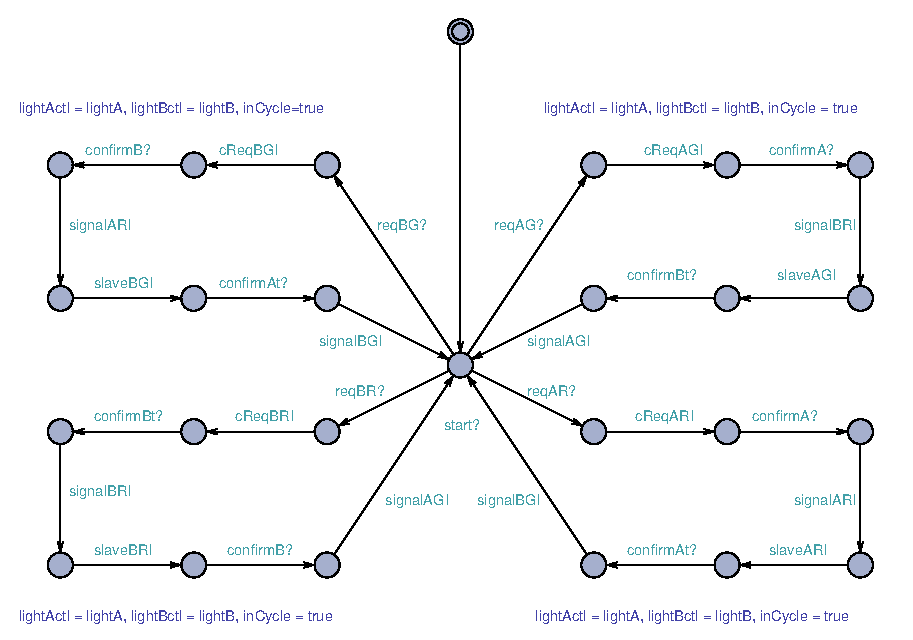
\includegraphics[width=4in]{res/MiddlewareModel.eps}}
\caption{Model of our Middleware in UPPAAL}
\label{fig:MiddlewareModel.eps}
\end{figure*}

Fig. \ref{fig:TrafficlightModel.eps} highlights the model of traffic lights and describes their behavior. The change of light's state is based on requests and confirmation exchange between lights and the middleware. We defined two roles for the traffic lights: one is set to master mode and the second one is set to slave mode.
Masters send requests every 60 seconds to change their states while considering the current ones. Line 6 of Algorithm \ref{Alg:traffic} shows the condition when a light should change its state. CLK state represents clock or time progress.  \emph{reqAG} and \emph{reqAR} are respectively the requests to ask for GREEN and RED states on road A. The same is specified for the road B.  
When it receives a confirmation from the middleware, a cycle is started to send the signal with the desired state. Every 30 seconds, the traffic lights can change their states, starting with GREEN light and then to YELLOW light for 3 seconds after that switching to RED. They can also start from RED and then change to GREEN state after additional 3 seconds. We add this extra delay to avoid a dangerous situation when a GREEN state is on the two roads A and B at the same time. Even if we have messages lost due to the wireless nature of the network, our UPPAAL models ensure that this situation doesn't arise. It has been introduced after experiencing a latency between the WSN and the Cloud platform (see section \ref{sec:Results}). When GREEN or RED states are actuated, confirmation messages are sent to the middleware. The pseudo Algorithm \ref{Alg:traffic} summarizes this mechanism.

\RestyleAlgo{algoruled}
\LinesNumbered \begin{algorithm}[ht] \caption{Traffic light\label{Alg:traffic}}
init\_60s\_timer();
	\While{true}{ \If{ end\_timer()}{ send\_request\_new\_state(); \\
	reset\_timer();
	}
\If{msg\_received\_red() and my\_state is green}{ change\_state(yellow);\\
	wait(); \\
	change\_state(red); \\
	send\_confirmation\_to\_middleware();
	}
\If{msg\_received\_green() and my\_state is red}{ change\_state(green);\\
	send\_confirmation\_to\_middleware();
	}
}
\end{algorithm}

% Figure
%\Figure{!htb}{1}{ControllerModel.png}{Model of our middleware in UPPAAL}


The model in Fig. \ref{fig:MiddlewareModel.eps} defines the different possibilities in terms of internal cycles depending on the request made by traffic lights (\emph{reqAG}, \emph{reqBG}, \emph{reqAR} \emph{reqBR}). Mainly, the middleware sends the message to the cloud and waits for its response. Then, it sends messages to traffic lights master and slave to change their state following this order: every light go to RED before setting GREEN signals. It also uses acknowledgments from the traffic lights to ensure that the new state has been set. In order to ensure these two features, we used a system to retain messages if the IoT Cloud Platform send GREEN states before RED states (see line 3 of Algorithm. \ref{Alg:conf} ). Algorithm \ref{Alg:conf} shows a simple description showing how the middleware confirms the order of traffic lights changes.


%By subscription, the middleware gets new states for the traffic lights and sends them accordingly to the master and slave traffic lights. It sends red states first and then green states to avoid unwanted behaviors. It also uses acknowledgments from the traffic lights to ensure that the new state has been set. In order to ensure these two features, we used a system to retain messages if the IoT Cloud Platform send green states before red states. Algorithm \ref{Alg:conf} shows how it works.

\RestyleAlgo{algoruled}
\LinesNumbered \begin{algorithm}[ht] \caption{Middleware confirmation\label{Alg:conf}}
\If{message\_received()}{ \If{ is\_green()}{ retain\_msg();
	//green then red }
\Else{ \If { retained\_msg\_exist()}{ update\_to\_red();
	//green then red }\Else{ update\_to\_red();
	//red then green }}
}
\While{true}{ confirmation\_red\_lights(); \\
	update\_to\_green(); \\
	confirmation\_green\_lights();
	}
\end{algorithm}
\begin{figure}[!htb]
\centering
\includegraphics[width=3.2in]{res/CloudModel.eps}
\caption{Model of our Cloud variables in UPPAAL}
\label{fig:CloudModel.eps}
\end{figure}


We introduced the IoT Cloud Platform model shown in Fig. \ref{fig:CloudModel.eps}. It simulates the subscription mechanism according to messages sent by the middleware to update collected data. We defined two states RED and GREEN without a transition state like YELLOW state defined for the traffic lights. The condition \emph{touchA} indicates if the road A detects the high priority vehicle. The name \emph{touch} is related to the type of sensor integrated in our prototype (see next section). The cloud confirms to the middleware that the state is changed by sending a message \emph{confirmA}. 

Exchanged messages within our WSN are based on IEEE 802.15.4 stack. And our middleware defines QoS levels of exchanged messages via MQTT protocol.  

%\RestyleAlgo{algoruled}
%\LinesNumbered \begin{algorithm}[ht] \caption{Middleware\label{Alg:middle}}
%initialization()\;
%	\While{true}{ \If{received\_red\_from\_roadA()}{ send\_msg\_to\_Cloud\_Platform();\\
%	confirmation\_msg(); \\
%	send\_red\_to\_roadA(); \\ get\_confirmation\_from\_roadA(); \\
%	send\_green\_to\_roadB(); \\ get\_confirmation\_from\_roadB(); \\
%	}
%% \If{received\_green\_from\_roadA()}{ send\_msg\_to\_Cloud\_Platform();
%confirmation\_msg();
%send\_red\_to\_roadB() get\_confirmation\_from\_roadB();
%send\_green\_to\_roadA() get\_confirmation\_from\_roadA();
%}
% \If{received\_red\_from\_roadB()}{ send\_msg\_to\_Cloud\_Platform();
%confirmation\_msg();
%send\_red\_to\_roadB() get\_confirmation\_from\_roadB();
%send\_green\_to\_roadA() get\_confirmation\_from\_roadA();
%}
% \If{received\_red\_from\_roadB()}{ send\_msg\_to\_Cloud\_Platform();
%confirmation\_msg();
%send\_red\_to\_roadB() get\_confirmation\_from\_roadB();
%send\_green\_to\_roadA() get\_confirmation\_from\_roadA();
%}
%}
%\end{algorithm}

% Figure
%\Figure{!htb}{1}{CloudModel.png}{Model of our Cloud variables in UPPAAL}




%At the end of that communication,
%	we have the IoT Cloud Platform showed in Figure \ref{fig:CloudModel.png}.
%We simulate the subscription mechanism,
%	according to the message sent by the middleware to update its own data.
%When modelization is done,
%the next step is to prototype it.

%\RestyleAlgo{algoruled}
%\LinesNumbered \begin{algorithm}[ht] \caption{Cloud\label{Alg:middle2}}
%\While{true}{ \If{ msg\_received\_green}{ variable\_to\_green();
%}
%\If{ msg\_received\_red}{ variable\_to\_red();
%}
%}
%\end{algorithm}

\section{Prototyping} \label{sec:Prototyping}

% Intro
We have prototyped the wireless sensors and actuator's network of traffic lights and roads on a mockup \footnote{https://github.com/IoT-UTLC/Resources/wiki} of real intersection in Paris with a scale of 1:68. Our specifications have been defined considering the low-cost and energy efficiency of the solution. This prototype is a proof of concept of not limited to our use case as it is scalable for other applications. For example, additional sensors of fine particules could be implanted bringing correlation between traffic jam and pollution. 
\begin{figure*}[!htb]
\centering
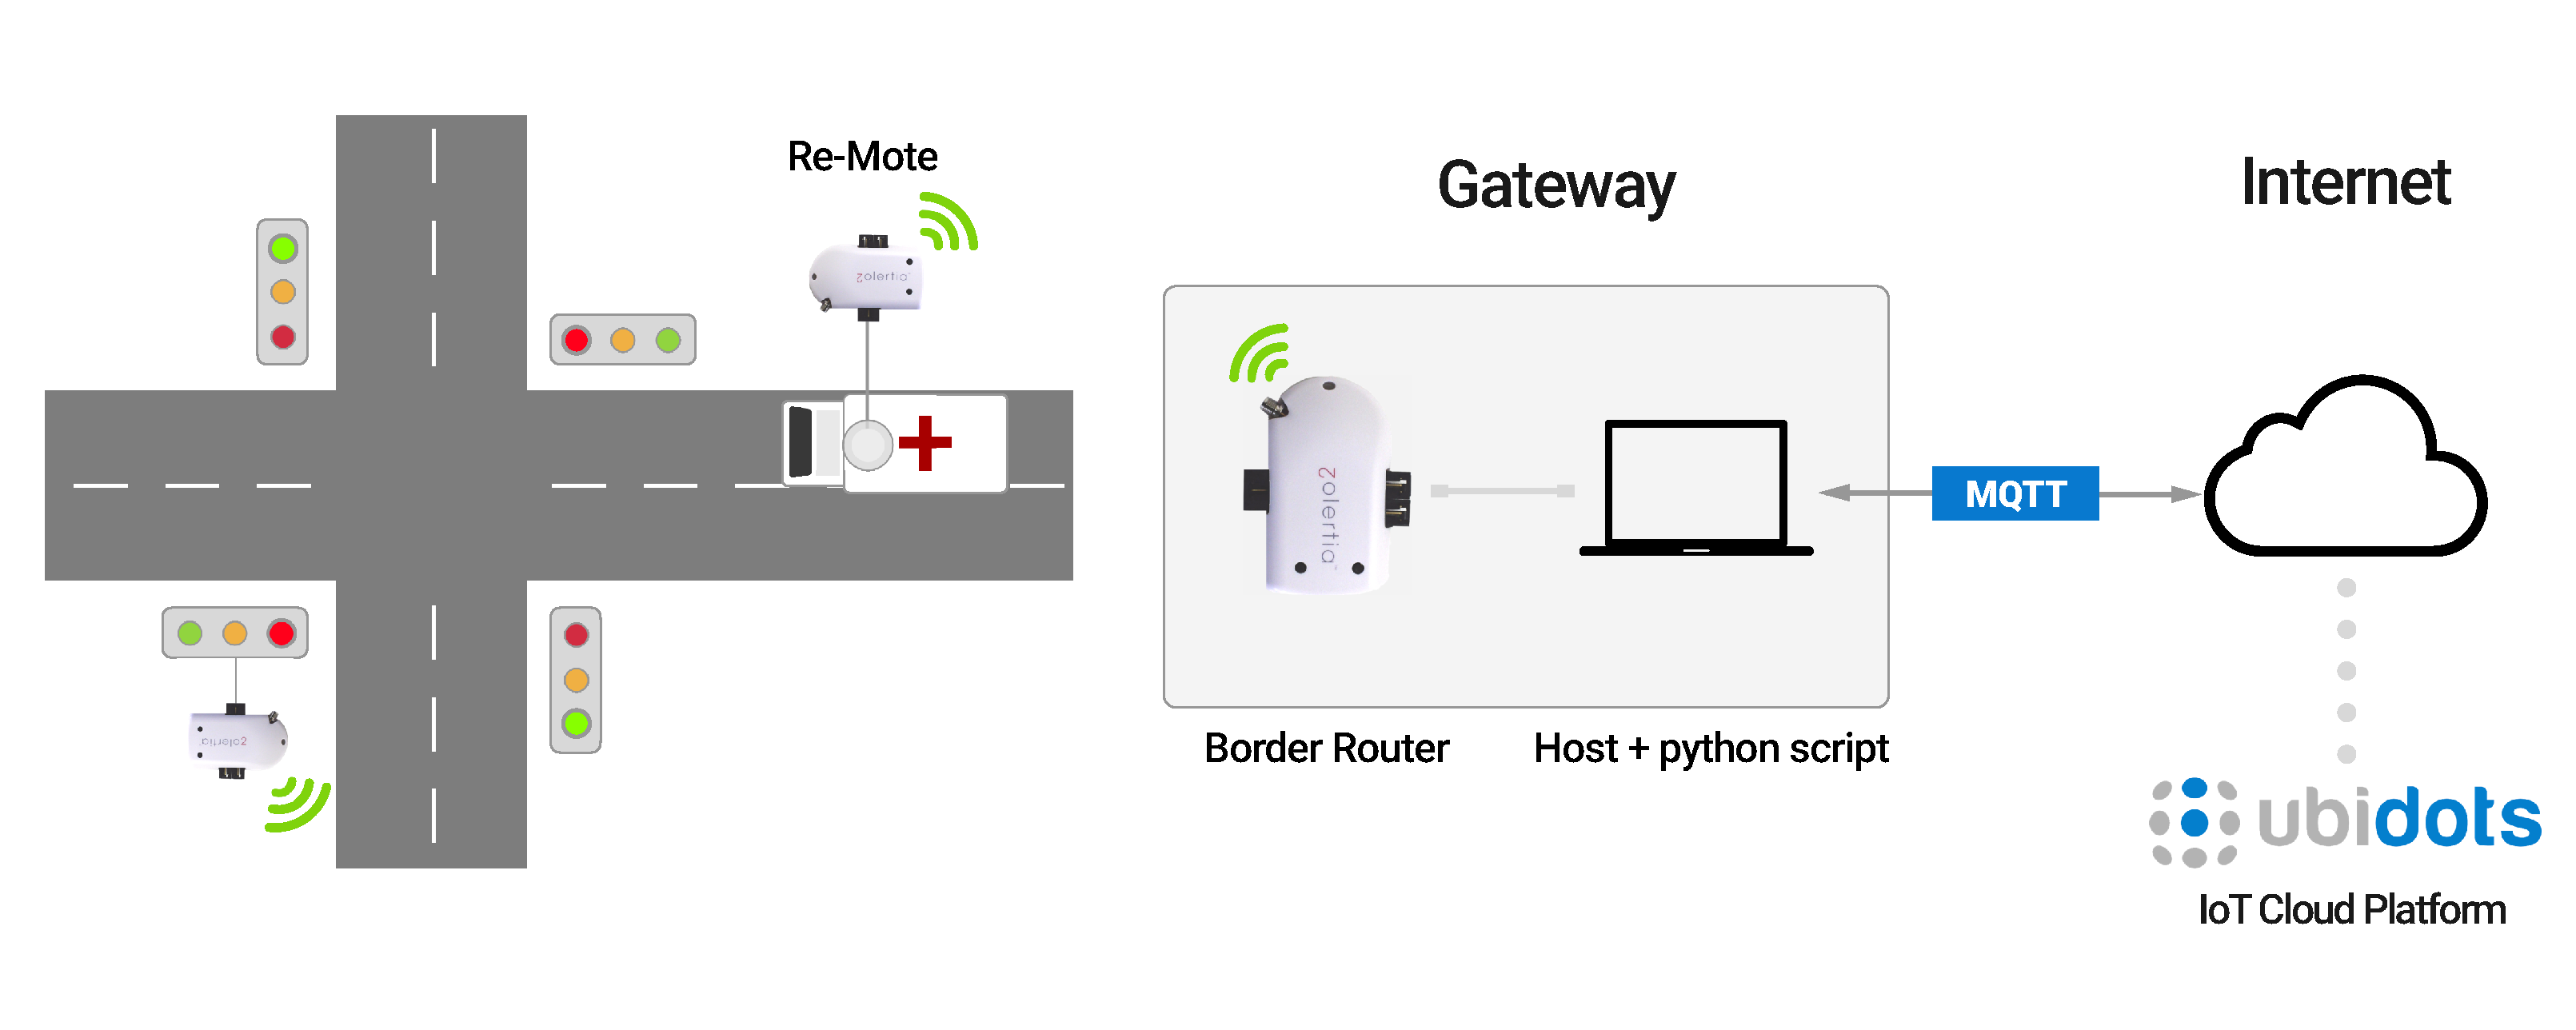
\includegraphics[width=4.5in]{res/ScenarioPaper.eps}
\caption{Architecture of  Iot-UTLC}
\label{fig:ScenarioPaper.eps}
\end{figure*}
%After defining what we are trying to achieve in this paper,
%	we focus on this section on technologies used to implement our project.
%% Defining every criterion and specifications we wanted Wireless Energy-efficient Portable
%One evident choice was to use a wireless solution.
%Indeed,
%	we want to avoid excessive costs and work on an existing crossroad for instance.
%We were looking for something portable to be placed on existing infrastructures and efficient depending on the situation.
%In addition, we wanted something that will not require a lot of power all the time, this is why we were looking for an energy-efficient device.

% Figure
%\Figure{!htb}{1}{ScenarioPaper.eps}{Architecture of our Iot-UTLC}

Fig. \ref{fig:ScenarioPaper.eps} shows the architecture of our IoT-UTLC with three layers. From left to right, we have the WSN layer with connected traffic lights’ actuators, sensors and IEEE 802.15.4 transceivers. The second part is the gateway of the WSN ensured by the BR and the middleware \emph{i.e.} Python scrip launched by host computer. 
The last layer is the Ubidots IoT Cloud Platform. It allows the system to collect WSN data. 



\subsection{6LoWPAN, Contiki OS, Re-Mote and Border Router} \label{Sec:Contiki}

% 6LoWPAN
Our WSN is an IPv6 LowPower Wireless Personal Area Network (6LoWPAN) based on IEEE 802.15.4 stack.
It is well adapted to embedded wireless devices with energy aware constraint and for its capabilities to define a mesh topology. Contiki Os\footnote{http://www.contiki-os.org/} has been used to implement networks' functions such as send, receive and data processing. 
It is an embedded operating system with large open source community. It supports Zolertia's Re-Motes \footnote{https://github.com/Zolertia/Resources/wiki/RE-Mote} and implements recent IEEE 802.15.4 standard specifications. It also includes protocols such as RPL, CoAP and MQTT. Furthermore, developer community is active and makes available source codes examples in order to help developing quickly new applications.

% Re-motes
Re-motes are compatible with our WSN specifications and our design model. They are wireless devices with ultra-low power operation mode. This choice has been motivated by long radio range of its IEEE 802.15.4 CC1200 transceiver, which transmits in the frequency band of 868-915 MHz. In addition, each Re-Mote has analog and digital ports with a possibility to connect several analog sensors and actuators. A Re-mote can be driven by a computer and become a sink and/or BR as well as a gateway between the 6LoWPAN network and the computer.

%\Figure{!htb}{1}{ethernetRouter.png}{Our Ethernet router}
\begin{figure}[!htb]
\centering
\includegraphics[width=2.5in]{res/ethernetRouter.png}
\caption{BR and sink combined on one board}
\label{fig:ethernetRouter.png}
\end{figure}
%[Explanation of how it works with the 2 radios,
To implement the previous model described in Section \ref{sec:Use Case and Model Design}, we used six Re-motes: one for the BR, four to control the traffic lights and one Re-Mote to detect the arrival of a high priority vehicle near a crossing point. For simplicity, we choose a touch sensor as a detecting device. We have developed four types of programs running on a Re-mote: traffic lights signs, sensors, high priority vehicle detecting device and BR function. Sensors send periodically information to the IoT Cloud Platform with temperature, pressure or any relevant information that can be sensed. As mentioned in the previous section, traffic lights are sub-divided into two modes: slaves and masters. Masters nodes are the only ones to request the middleware to change its light’s state and slaves simply change its state depending on received packets. These roles are defined to reduce the overhead of network, redundancy and collisions, for instance. Masters send periodically packets to request a change of state to the middleware which forwards them to a cloud platform.



% Border router

 
BR node behaves differently compared to the other Re-motes. The entries of its routing table are the list of Re-motes that pass through it. It reroutes every packet it receives from its neighboring to host computer (or sink), which  creates a connection to the IoT Cloud platform. Two options are possible to create our BR: i) separate the BR and sink and ii) combine both on the same device. 
In our development, we worked on how to implement the sink and the BR nodes on the same Re-Mote board. Fig. \ref{fig:ethernetRouter.png} shows a prototype of the combined BR and sink, both connected to an ethernet interface. Indeed, if the border router becomes an Ethernet router, there will no longer be any connection between the host/sink machine and the IoT Cloud platform. Every Re-mote is able to connect independently to the IoT Cloud platform. This approach has some advantages, such as the autonomy of the devices, but it generates an overhead requiring extra synchronization packets' exchange. Therefore, we separate the sink and BR, since this solution is more flexible and resilient for our prototype.

%The border router is at first a Re-mote,
%	but it has very different behavior and function.
%Indeed it has the task of re-routing every packet it receives from its cohorts to the serial port of the host machine.


%This machine will create a connection to the IoT Cloud platform and send the Re-motes messages to it and get responses for the Re-motes.
%The border router is a central node because it knows all to Re-motes in the 6LoWPAN which packets have transited by it.
%It acts as a Router and has a routing table of those Re-motes that pass through it.
%A web server page can be accessed to retrieve that information.
%We also tried a different approach of it.

 % [
%Transition with next paragraph => the use of MQTT to access the other "side" of the system
%Explanation of how it works (encapsulating the headers ...)
%]
%[
%Big part of how it works,
%what is good about it %New paragraph about the autonomous BR we were trying to develop
%Comparison between the 2 solutions
%]

% Autonomous BR
%As we have seen before,
%	this approach requires a Border Router linked the computer itself to the internet,
%	we tried to see if we can remove one part.
%Thus,
%	we added a component to the Re-mote in order to connect it directly to the internet via an Ethernet cable.

%[Transition with next paragraph => the use of MQTT to access the other "side" of the system]

\subsection{MQTT and UBIDOTS} \label{Sec:MQTT}

After establishing the access network of WSN, the next step is to connect this network to Core network (the Internet cloud platform). MQTT protocol controls three levels of QoS of exchanged packets from the WSN to the chosen Ubidots \footnote{https://ubidots.com/} cloud platform. It adopts IntServ approach for supporting quality of service in the network,
	it tags incoming packets in the border routers with different levels of priority.
Core routers read incoming packets headers and queue them according to their priority,
	packets with a high priority are sent faster compared to low priority ones.

MQTT ensures the QoS and publish/subscribe mechanisms through a broker. The broker behaves as a server by filtering messages and organizing them in topics, which are strings used to filter messages and define the hierarchy of our data structure. 
They allow us to organize how to receive multiple data from sensors such as temperature, up time, battery status and how to display them and obtain a real-time glance of our system.  It gets its messages from publishers and sends any modifications to entities, which that subscribed to the updated topics. We used this mechanism with the middleware in order to publish messages to the broker and get from the main topic the new values of the subscriber.

%We have seen in previous section what we used for our local sensors network, let's see now how we communicate with the IoT Cloud Platform. We will use MQTT which is a light-weight transportation protocol. In our solution, a python script will run an MQTT client to connect our WSN to Ubidots.


%MQTT ensures the QoS and publishes/subscribes mechanisms with a noteworthy topic organization. 

%The topics are strings used to filter messages and define the hierarchy of our data structure. They allow us to organize how to receive multiple data from sensors such as temperature, up time, battery status and how to display them and obtain a real-time glance of our system. 

%In addition, the broker behaves as a server by filtering messages and organize them in topics. It gets its messages from publishers and will send any modifications to entities which would have subscribed to the updated topics. We used this mechanism with the middleware in order to publish messages to the broker and get from the main topic the new values using the subscriber functionality.


The QoS feature of MQTT protocol manages network resources by handling retransmissions and guarantees the delivery of messages. It allows more control on messages by defining the level of guarantee. By default, the QoS is defined by three levels. The first one, level 0, is `At most one`. Level 1 is `At least one` where there is an acknowledgment to let the sender know that its packet has been received. Finally, level 2 `Exactly once` is the highest verification level with a request/response flows to ensure that only one message will be delivered and processed by the receiver. In our case, we applied levels 1 and 2 using \textit{paho.mqtt.client} Python library.  
%
%For example, subscribed clients could define the data QoS level of requested data by the source code shown bellow. 
For example, publisher of high priority data such as touch sensor has to indicate the highest level of QoS by the code shown bellow. 
We shared our implementation and its source codes at https://github.com/IoT-UTLC/contiki.
%
%\begin{footnotesize}
%\begin{lstlisting}
%# client receives a CONNACK response 
%# from the server.
%def on_connect(client, userdata, flags, rc):
%  print("Subscribed to " + MQTT_URL_TOPIC)
%  client.subscribe(MQTT_URL_TOPIC, 2) 
%  # 2nd arg is the QoS level to use 
%  # at maximum when it's needed
%\end{lstlisting}
%\end{footnotesize}

\begin{footnotesize}
\begin{lstlisting}
payload = json.dumps({"RoadA": data, "RoadB": 0})
res, mid = conn.publish(MQTT_URL_PUB, payload,
	  qos=int(QoS)) # QoS is QoS level to use 
\end{lstlisting}
\end{footnotesize}


%# The callback for when the client receives a CONNACK response from the server.
%def on_connect(client, userdata, flags, rc):
%	print("Connected with result code "+str(rc))
%	print("Subscribed to " + MQTT_URL_TOPIC)
%	client.subscribe(MQTT_URL_TOPIC, 2) 
                                                                                                                                                        
We experienced significant latency of high priority messages when we did our first tests of IoT-UTLC mockup. Therefore, assessments of the MQTT protocol in our case provided significant information about its efficiency. 

%  For the end point the IoT Cloud platform,
% we wanted to be simple  %QoS and MQTT resilient by default (good implementation)
% Get relevant information from dashboard
% Access from anywhere (remote control possible)
% Structure our system / hierarchy
%
%As for the MQTT broker, we wanted an easy and powerful IoT Cloud Platform.
%It will be compatible with all technologies we chose for our prototyping,
%	so with an integration of MQTT and QoS levels.
%an IoT Cloud platform is a central point of the system as it keeps all the information about our WSN.
%Using the Cloud allows the system being accessible from anywhere on the internet.
%It is also a tool to filter and display relevant information in real-time from our system in the centralized dashboard.
%It can be possible to trigger some actions on the system via the dashboard.
%
%% Architecture
%Building this virtual infrastructure for this project has been challenging.
%we used MQTT topics mechanism to get the most of Ubidots to structure every data sent.
%We have a main topic which contains the states of the traffic light (RoadA and RoadB) in real time,
%	we created individual topics for every Re-mote acting as traffic lights or sensors.
%With this architecture,
%	we can have deep information on every device (such as its battery,
%	sensors data,
%	etc...).
%Moreover,
%	it could be scaled to match future needs.

\section{Results} \label{sec:Results}

% Methodology
In this section, we report experimental results of urban traffic-light control system based on MQTT protocol. We report the limitations of our solution. To test the efficiency of MQTT protocol, we made 2 scenarios, in the first scenario, the frequency  packets sending  is 1 packet per 10s, the second scenario, the frequency  packets sending  is 1 packet per 1s. The measured delays have been taken into account between the middleware to the cloud platform (Ubidots) throughout the Internet. Note that we don't know the routes and the routers that our packets will go through. We measured the Round Trip Time (RRT) for the packets exchanged between the two sides. In each scenario, more than 100 values have been taken. Tests have been reproduced for two different hours and days.


%\Figure{!htb}{1}{cdf_distribution.pdf}{Normal,Gamma and Logistic distribution}
\begin{figure}[!htb]
\centering
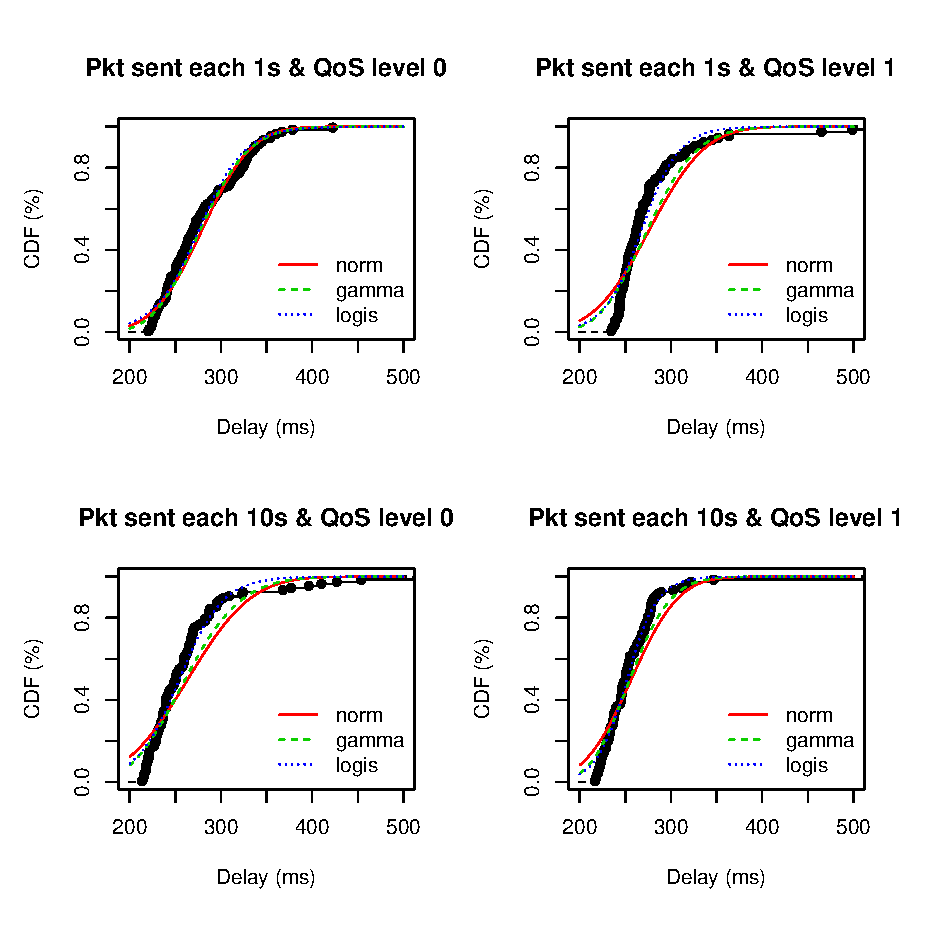
\includegraphics[width=\columnwidth]{res/distributions_v3.eps}
\caption{Normal, Gamma and Logistic distribution}
\label{fig:cdf_distribution.pdf}
\end{figure}

Fig. \ref{fig:cdf_distribution.pdf} shows the measured Cumulative Distribution Function (CDF) of RTT delays for the two levels of QoS, levels 1 and 2. We consider three probabilistic distribution functions (Normal, Gamma and Logistic) in the experimental results in order to characterize MQTT performance. The obtained correlation allows us to define a representative empirical model. Table \ref{table:correlation} details the results of a correlation matrix between distributions and experimental results. We can see that logistic distribution \cite{STEPHENS1979} fits better with our measured RTT values for the two scenarios. The standard logistic law is of parameters 0 and 1. Its distribution function of a random variable $x$ is the sigmoid following the expression:

\begin{equation}
F(x) = \frac{1}{1 + e^{-x}} \mbox{,where } x\in \left[ -\infty, +\infty\right]
\end{equation}
%\Equation{1}{F(x) = \frac{1}{1 + e^{-x}} \mbox{, where } x\in \left[ -\infty, %+\infty\right] } 




%Results show that packet delays in both scenarios with the level of QoS match better the logistic distribution than the tow other distributions.
%
%\blue{To study the behavior of packet delays in each scenario,
%	we select the best distribution that fit the round trip time (RTT) of packets,
%	we choose 3 common distributions normal,
%	gamma and logistic distribution shown in figure \ref{fig:cdf_distribution.pdf}.
%Table \ref{table:correlation} shows the correlation matrix between distributions and scenarios used in our study.
%Results show that packet delays in both scenarios with the level of QoS match better the logistic distribution than the tow other distributions.
%The standard logistic law is the logistic law of parameters 0 and 1, its distribution function is the sigmoid: 
%\Equation{1}{F(x) = \frac{1}{1 + e^{-x}}}
%}

\begin{table} [!htb]
\caption{Correlation between distributions and empirical results}
\centering
  \begin{tabular}{ | c | c | c | c | }
    \hline
	\                    & norm      & gamma    & logis         \\\hline 
	1s  with QoS level 1 & 172.12074 & 175.2950 & \bf{185.4433} \\\hline 
	1s  with QoS level 2 & 159.59630 & 172.8193 & \bf{189.7002} \\\hline 
	10s with QoS level 1 & 146.85668 & 161.2369 & \bf{175.3682} \\\hline 
	10s with QoS level 2 & 176.28502 & 192.6108 & \bf{204.3235} \\\hline
  \end{tabular}
\label{table:correlation}
\end{table}

%\Table{|c|c|c|c|}{correlation}{Matrix of correlation between distribution and empirical results }{
%	\                    & norm      & gamma    & logis         \\\hline 
%	1s  with QoS level 0 & 172.12074 & 175.2950 & \bf{185.4433} \\\hline 
%	1s  with QoS level 1 & 159.59630 & 172.8193 & \bf{189.7002} \\\hline 
%	10s with QoS level 0 & 146.85668 & 161.2369 & \bf{175.3682} \\\hline 
%	10s with QoS level 1 & 176.28502 & 192.6108 & \bf{204.3235} \\\hline
%}

% Figure
%\Figure{!htb}{.9}{cdf.pdf}{Cumulative distribution function of RTT delay}
\begin{figure}[!htb]
\centering
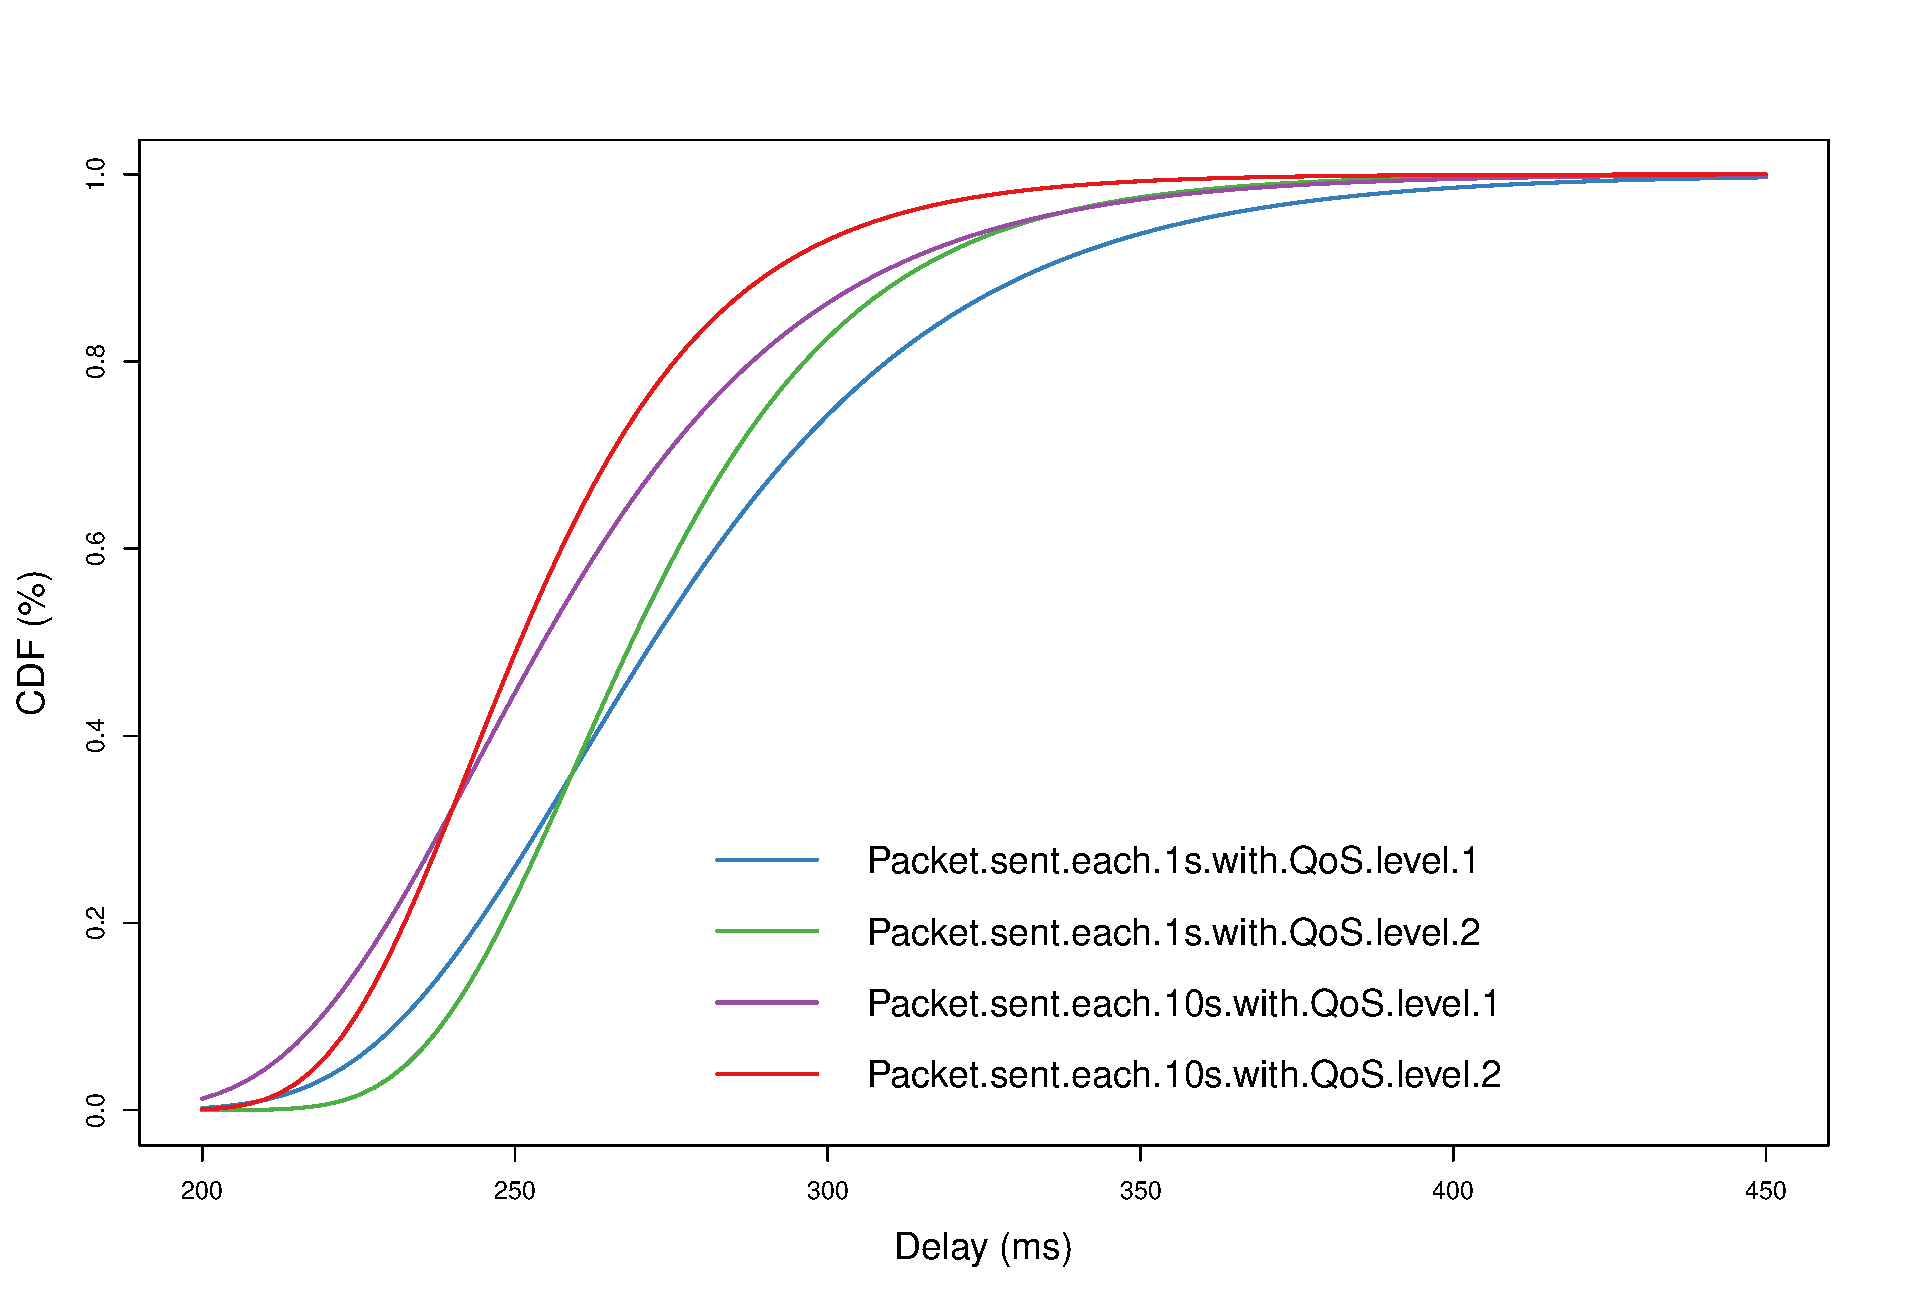
\includegraphics[width=3.5in]{res/cdf_v3.eps}
\caption{Cumulative distribution function of RTT delay for two QoS levels}
\label{fig:cdf.pdf}
\end{figure}

Fig. \ref{fig:cdf.pdf} highlights the empirical model of CDF featuring the RTT of MQTT protocol. As can be seen, RTT protocol is more efficient when the number of packets is greater than 35\% of the total number of packets sent. This can be explained by the fact that priority queues are useful when queues of QoS are full. In that case, the packets with a highest priority level will reach their destination with low latency. Furthermore, when we increase the number of packets sent to Ubidots at one per second, the MQTT still offers the same efficiency with suitable delays. The found latency of up to 400 ms would be problematic for real world safety applications which require at most 100 ms \cite{Chen2017}.

Although our Mockup is innovative by combining IEEE 802.15.4, 6LowPAN and MQTT protocol, the performances of our solution depend on external parameters.  These parameters are related to Internet Service Provider and all packet's routes throughout Internet network from the middleware to Ubidots. Thus, real implementation of such a system should be done taking into account all sources of latency. 

%\blue{ Figure \ref{fig:cdf.pdf} shows that the MQTT protocol is more efficient when the number of packets is greater than 35\% of the total number of packets sent,
%this can be explained by the fact that priority queues are more useful when all levels of queues are filled,
%	so the packets with a high priority level will achieve their destination faster.
%% Performance
%Moreover,
%	when we tried to increase the number of packets sent to Ubidots at one per second,
%	the MQTT still offers the same efficiency with suitable delays.
%}

\section{Conclusion} \label{Sec:Conclusion}

%%%%%%%%%%%%%%%%%%%%%%%%%%%%%%%%%%%%%%%%%%%%%%%%%%%%%%%%%%%%%%%%%%%%%%% Restate the main challenges %%%%%%%%%%%%%%%%%%%%%%%%%%%%%%%%%%%%%%%%%%%%%%%%%%%%%%%%
In this paper, we proposed a Urban Traffic Light Control (IoT-UTLC), considering its architecture’s elements and tools used to build an IoT mockup.
We reported three main contributions in this work: i) Modelling through UPPAAL of crossing's traffic lights ii) Prototyping of IoT network and iii) Performance assessment of MQTT protocol. Traffic lights control has been taken as an IoT network. WSN has been deployed on motes running Contiki Os and exchanging IEEE802.15.4/6LowPAN packets. MQTT was the QoS protocol between our WSN and Ubidots cloud platform. UPPAAL model checker design ensured that lights' colors change is adaptive to the arriving of a priority vehicle.
%%%%%%%%%%%%%%%%%%%%%%%%%%%%%%%%%%%%%%%%%%%%%%%%%%%%%%%%%%%%%%%%%%%%%%% Restate the main contribution %%%%%%%%%%%%%%%%%%%%%%%%%%%%%%%%%%%%%%%%%%%%%%%%%%%%%%
%Of course, the IoT solution would be useful to interconnect heterogeneous network technologies. 
%We see that IoT could platforms are useful to interconnect different network technologies by supporting more dynamic use cases in UTLC systems.

%%%%%%%%%%%%%%%%%%%%%%%%%%%%%%%%%%%%%%%%%%%%%%%%%%%%%%%%%%%%%%%%%%%%%%% Restate the main findings %%%%%%%%%%%%%%%%%%%%%%%%%%%%%%%%%%%%%%%%%%%%%%%%%%%%%%%%%%
Our experiments have investigated the relationship between the MQTT protocol and the traffic flow congestion. Our results showed that the MQTT is efficient when the number of packets sent exceeds 35\% of the total number. The packets with highest level of QoS has low latency than other packets. The protocol remains efficient since the delay of priority packets decreases when the network overhead increases. However, found latencies of up to 400ms is higher than the expected one for vehicular safety application. Thus, the proposed IoT architecture and protocols must be improved to consider the safety requirements. 
%%%%%%%%%%%%%%%%%%%%%%%%%%%%%%%%%%%%%%%%%%%%%%%%%%%%%%%%%%%%%%%%%%%% Future challenges current bad state %%%%%%%%%%%%%%%%%%%%%%%%%%%%%%%%%%%%%%%%%%%%%%%%%%
While we are still developing our prototyping, we plane to integrate other use cases such as smart buildings and industrial IoT.
% Improvements
As a near future work, we plane to extend our experiments to measure both delay and Packet Delivery Ratio (PDR).

\section*{Acknowledgement}

We would like to thank our colleague Sebti Mouelhi, associate professor at ECE Paris, who provided us insight and expertise on UPPAAL.


\bibliographystyle{IEEEtran}
\bibliography{biblio}



% that's all folks
\end{document}
